\chapter{Experimental Results}

In this section, we provide experimental results from our tool
on several code-breaking games.
In the tables below, MM($n$,$m$) refers to Mastermind with $n$ pegs and $m$ colors,
CC($n$) refers to the counterfeit coin problem with $n$ coins,
BG($n$,$m$) refers to problem Bags of gold with $n$ bags and balance scale capacity $m$.
SM($n$,$m$) refers to the Mastermind variant with black markers only, i.e.
  for each guess, the codebreaker gets the number of positions at which the code
  and the guess match.

\section{Performance}

All experiments have been run on Intel Core i7-3770 3.40GHz and COBRA was
compiled with \texttt{gcc} 4.8.2.
The symmetry breaking engine has been turned off for this section,
  so that we can compare the actual performance of the SAT solvers.

\autoref{tbl:exp-sat-wellformed} lists running times of well-formed check for sample games.
Naturally, proper SAT solvers are orders of magnitude faster than simple solver
as well-formed check is based on verification of unsatisfiability of a large formula.

\begin{table}[h]
\begin{center}
\begin{tabular}{|l|c|c|c|c|} \hline
Game & Simple / s & Minisat & Picosat  & \# calls \\ \hline
MM(4,6) & 174 & 2.7 & 3.2 & 1296 \\
MM(5,4) & 217 & 14.3 & 34.8 & 1024 \\
BG(12,12) & 3539 &  0.5 & 1.1 & 271 \\\hline
\end{tabular}
\caption{Running times (in seconds) of well-formed check.}
\label{tbl:exp-sat-wellformed}
\end{center}
\end{table}

\autoref{tbl:exp-sat-sim} \TODO{...}

\begin{table}[h]
\begin{center}
\begin{tabular}{|l|c|c|c|c|} \hline
Task & Simple & Minisat & Picosat & \# calls \\ \hline
Select first exp. (parts) & 3.9 & 2.6 & 523 & 17,108 \\
Select first exp. (max-models) & 9.3 & 45.3 & $>$ 5000 & 3145 \\
Simulate (parts $\times$ models) & 15.1 & 32.3 & 3024 & 31,061 \\
Simulate (max-models $\times$ models) & 10.5 & 7.9 & 749 & 92,644 \\\hline
\end{tabular}
\caption{Running times (in seconds) of simulation and strategy evaluation on MM(4,6).}
\label{tbl:exp-sat-sim}
\end{center}
\end{table}

\autoref{tbl:exp-sat-analyse}
  shows total running times and number of calls to
  a SAT solver during strategy analysis.
A clear winner in this case is the simple solver based on
  model enumeration,
  which is not unexpected.
On lower levels of the backtracking algorithm,
  the analysed formulas has only few models and the
  overhead with calling a proper SAT solver is bigger
  than simply going though all potential models and verifying whether
  they are satisfied.

The results also show that questions on number of models
  are much harder than satisfiability questions.
For the simple solver, the difference is not that significant,
  but our simple and unoptimized model counting algorithm
  takes much longer.
That is the reason why the analysis of strategy ``parts'' is usually much faster
  than analysis of strategy ``max-models''.

With simple solver, however, analysis of ``max-models'' is faster than
  analysis of ``parts''. \TODO{Protoze to muzu rychlej useknout..}

\begin{table}
\begin{center}
\begin{tabular}{|l|l|c|c|c|c|} \hline
Game & Strategy& Simple / s & Minisat / s & Picosat / s & \# calls \\ \hline
MM(3,4) & parts & 0.1 & 0.4 & 13.5 & 13,769 \\
MM(3,4) & max-models & 0.1 & 2.1 & 179 & 9,349 \\
MM(3,4) & exp-fixed & 0.3 & 17.4 & 1974 & 15,002 \\
MM(4,4) & parts & 6.9 & 237 & $>$ 5000 & 260,144 \\
MM(4,4) & max-models & 5.0 & 1126 & $>$ 5000 & 188,828 \\
MM(4,4) & exp-fixed & 24 & $>$ 5000 & $>$ 5000 & 329,820 \\
CC(20) & parts & 0.1 & 0.3 & 12.8 & 7,718 \\
CC(20) & max-models & 0.2 & 28 & 3161 & 12,117 \\
CC(20) & exp-fixed & 0.3 & 73 & $>$ 5000 & 14,273 \\\hline
% Analyse parts & CC(30) &  6.87 & 237 & ? & 260,144 \\
% Analyse parts & CC(30) &  0.08 & 0.34 & 13.5 & 13,769 \\
% Analyse max-models & CC(30) & ? & ? & ? & ? \\
% Analyse max-models & CC() & ? & ? & ? & ? \\
\end{tabular}
\caption{Running times (in seconds) of strategy analysis.}
\label{tbl:exp-sat-analyse}
\end{center}
\end{table}


\section{One-step look-ahead strategies}

In this section, we compare performance of one-step look-ahead strategies
defined in \autoref{sec:oslas}.

\subsection{Counterfeit coin problem}

The average-case number of experiments performed by one-step look-ahead
  strategies in the counterfeit coin problem
  for the number of coins from 3 to 40 is shown in \autoref{fig:exp-cc}.

Notice that bigger number of coins does not necessarily mean that
  identifying the counterfeit coin is more difficult.
For example, for 16 coins, the ``max-models'' strategy needs
  3.44 experiments on average but for 17 coins it is only 3.41.
That is because the additional coin changes
  the numbers of models for some outcomes,
  which may lead to better experiment selection.

Interestingly, ``exp-fixed'' strategy outperforms all others
  on 20, 21, 23, 25 and 27 coins, while it seems to be
  generally worse.
Strategies ``parts'' and ``min-fixed'' are clearly unsuitable for
  a problem of this kind.

\begin{figure}[h]
\begin{center}
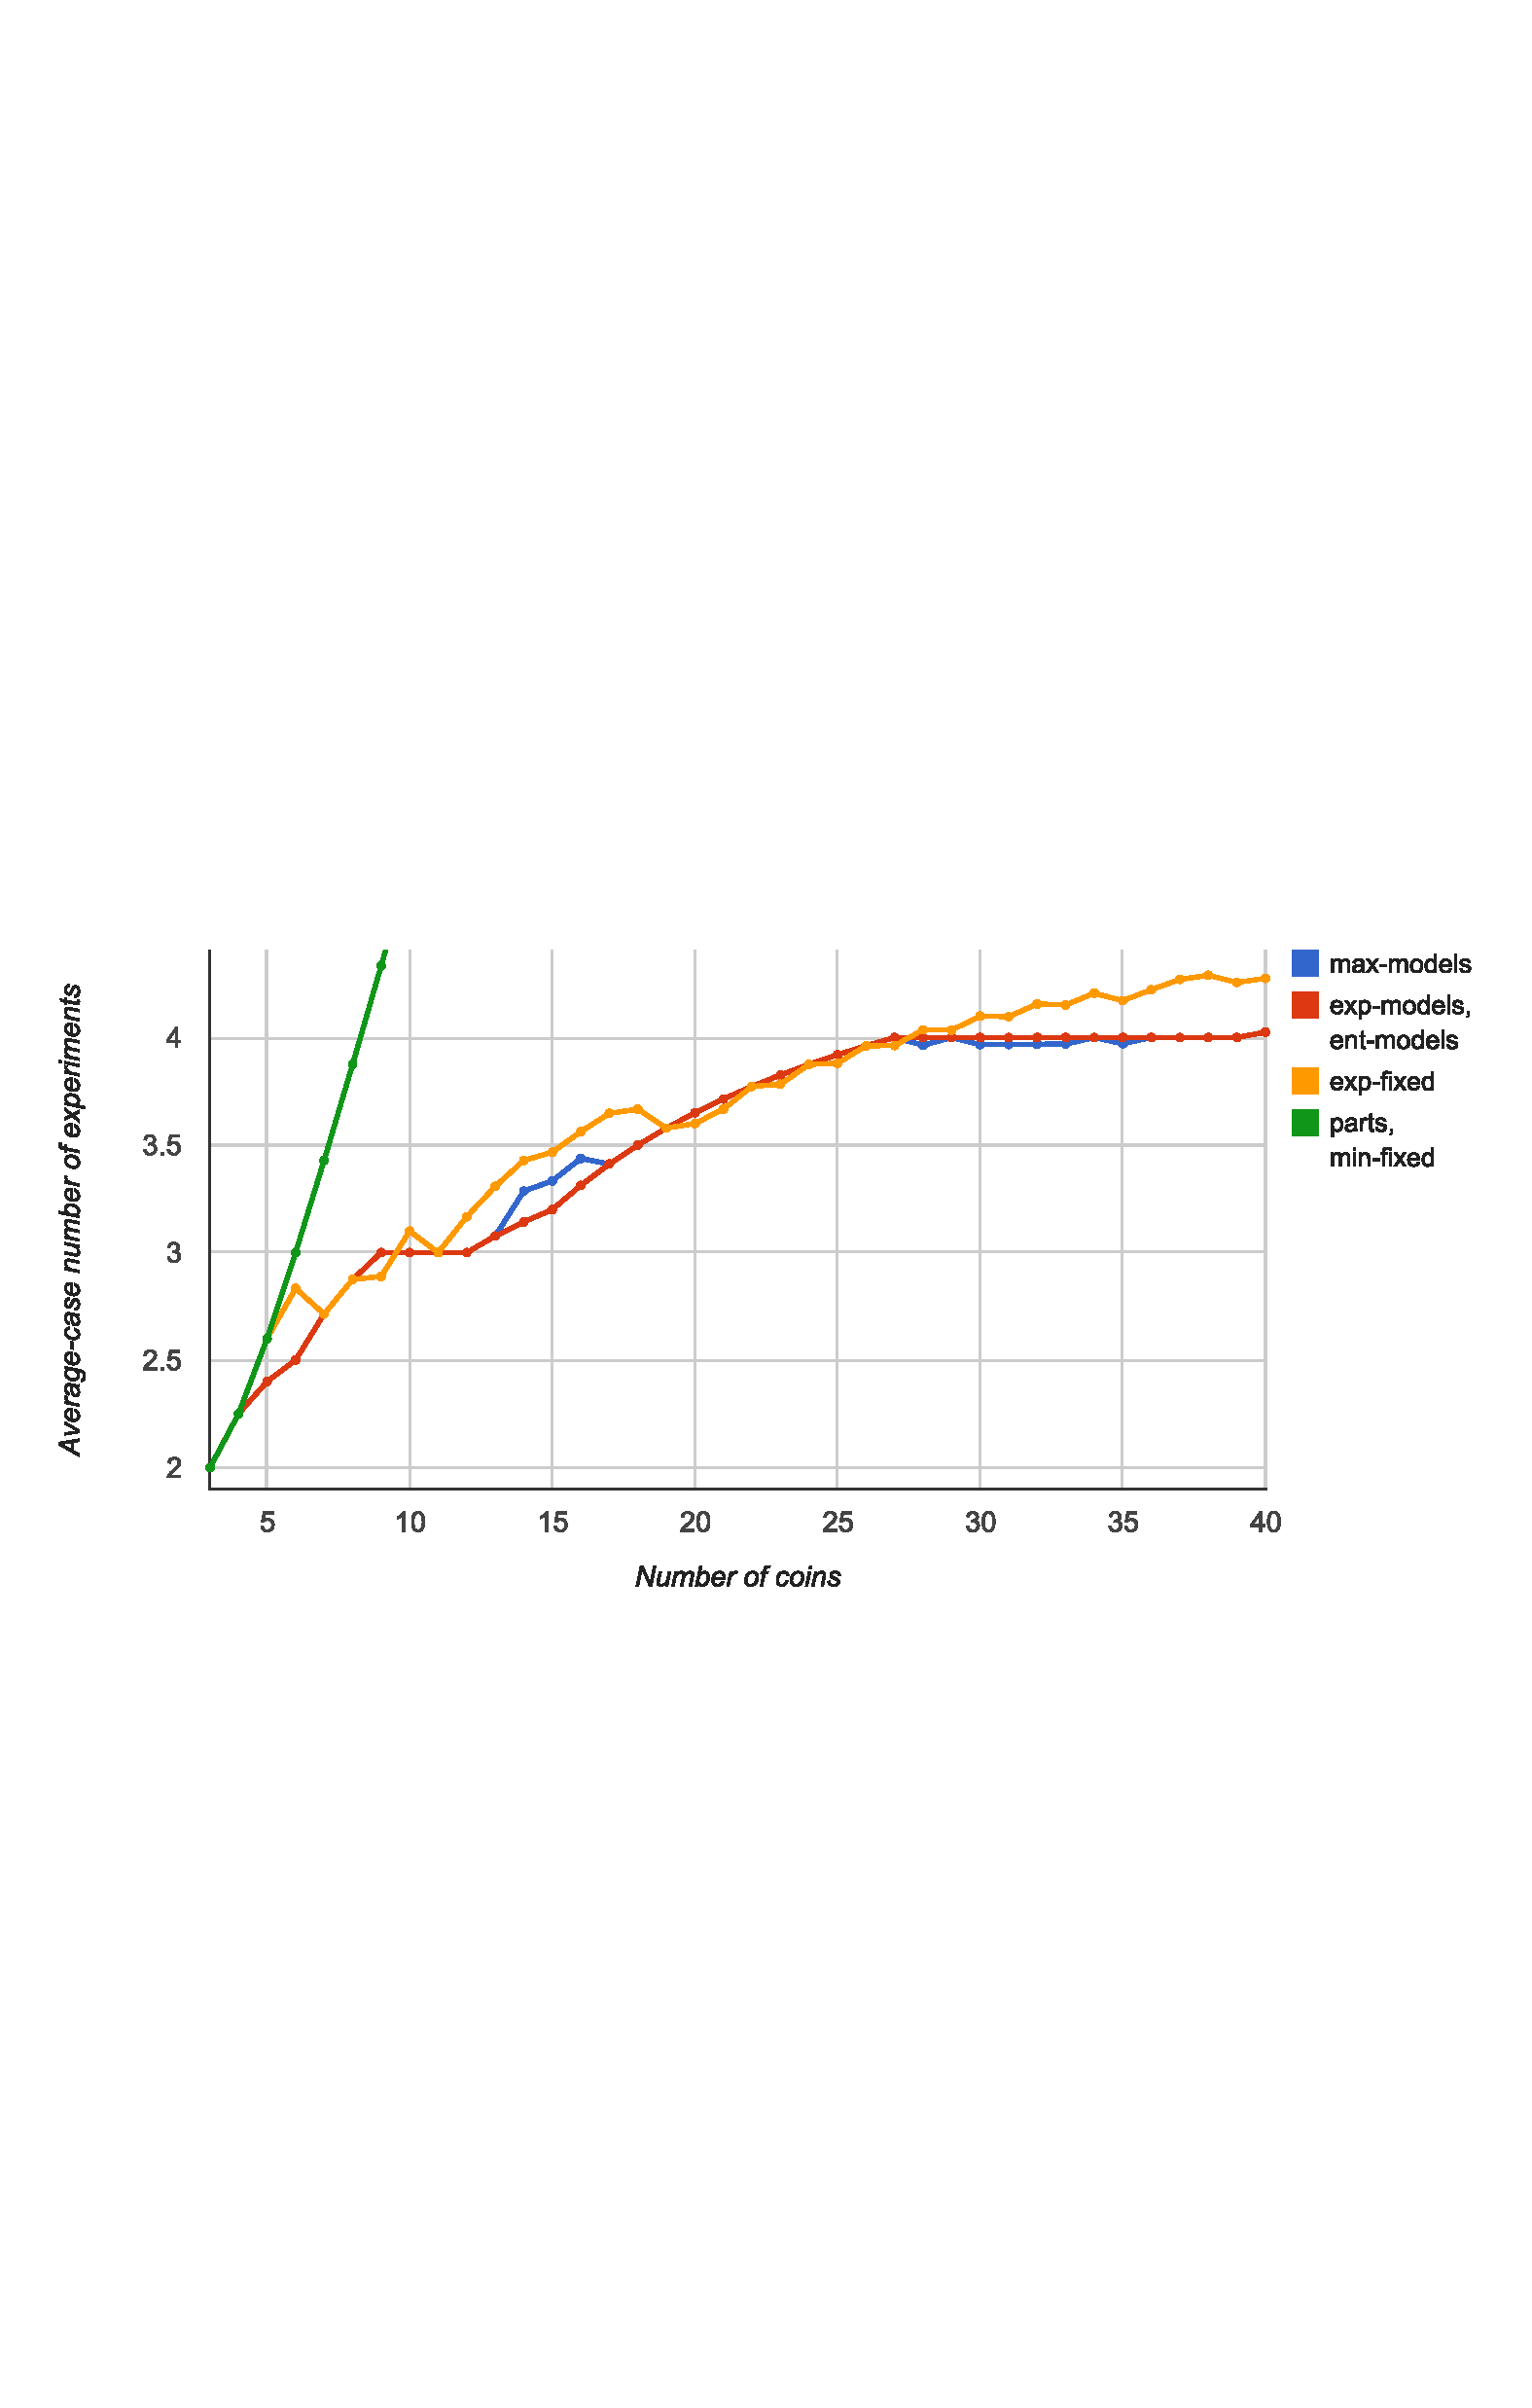
\includegraphics[width=\textwidth]{pictures/graph-cc.pdf}
\caption{Average-case number of experiments in the counterfeit coin problem.}
\label{fig:exp-cc}
\end{center}
\end{figure}

\subsection{Mastermind}

Results for Mastermind are shown in \autoref{tbl:exp-mm}.
A clear winner in the average-case number of experiments is the ``parts'' strategy,
followed by ``max-models''.

In the worst-case number of experiments, ``max-models'' outperforms other
  strategies in all cases except for MM(3,2).
This case was already mentioned in \TODO{..};
the strategy needs four steps due to an ``unlucky'' choice of the first experiments.

Again, notice that bigger size of the problem does not necessarily mean that
  revealing the secret is harder, as can be seen on the values for MM(5,2) and MM(5,3).

\begin{table}[h]
\begin{center}
\begin{tabular}{|c|c|c|c|c|c|c|c|c|c|c|c|c|}\hline
Game & \multicolumn{2}{c}{max-mod} & \multicolumn{2}{c}{parts}
& \multicolumn{2}{c}{exp-mod} & \multicolumn{2}{c}{ent-mod}
& \multicolumn{2}{c}{min-fix} & \multicolumn{2}{c}{exp-fix}\\ \hline
MM(2,3) & 2.667 & 4 & 2.333 & 3 & 2.444 & 3 & 2.444 & 3 & 2.667 & 4 & 2.444 & 3 \\
MM(2,6) & 3.667 & 5 & 3.667 & 5 & 3.861 & 5 & 3.861 & 5 & 4.611 & 7 & 4.167 & 6 \\\hline
MM(3,2) & 2.625 & 4 & 2.250 & 3 & 2.250 & 3 & 2.250 & 3 & 2.625 & 4 & 2.25 &  3 \\
MM(3,6) & 4.046 & 5 & 3.977 & 5 & 4.227 & 5 & 4.218 & 5 & 5.259 & 8 & 4.546 & 6 \\
MM(3,8) & 4.787 & 6 & 4.701 & 6 & 4.879 & 6 & 4.844 & 6 & 6.688 & 10 & 5.631 & 8 \\\hline
MM(4,2) & 2.750 & 4 & 2.750 & 4 & 3.063 & 4 & 3.063 & 4 & 3.250 & 5 & 3.063 & 4 \\
MM(4,6) & 4.476 & 5 & 4.374 & 6 & 4.626 & 6 & 4.643 & 6 & 5.765 & 9 & 5.231 & 7 \\
MM(4,7) & 4.837 & 6 & 4.743 & 6 & 4.962 & 6 & 4.947 & 6 & 6.476 & 10 & 5.945 & 8 \\
MM(4,8) & 5.183 & 6 & 5.102 & 7 & 5.293 & 7 & 5.272 & 7 & 7.213 & 11 & X & X \\\hline
MM(5,2) & 3.500 & 5 & 3.313 & 5 & 3.938 & 5 & 3.625 & 5 & 3.875 & 6 & 3.781 & 5 \\
MM(5,3) & 3.407 & 4 & 3.379 & 4 & 3.634 & 4 & 3.609 & 4 & 4.444 & 7 & 3.942 & 5 \\
MM(5,4) & 3.991 & 5 & 3.880 & 5 & 4.092 & 5 & 4.083 & 5 & 5.014 & 9 & 4.617 & 6 \\\hline
\end{tabular}
\caption{Average-case and worst-case number of experiments\\
  of one-step look-ahead strategies in Mastermind.}
\label{tbl:exp-mm}
\end{center}
\end{table}


\subsection{String matching (Mastermind with black markers only)}

Mastermind with black markers only is an example of a game,
  where ``max-models'' does not perform so well.
Exact values are shown in \autoref{tbl:exp-mmb}.

A winner in this case is the strategy based on entropy of the number of models,
  closely followed by ``parts'' strategy.

\begin{table}[h]
\begin{center}
\begin{tabular}{|c|c|c|c|c|c|c|c|c|c|c|c|c|}\hline
Game & \multicolumn{2}{c}{max-mod} & \multicolumn{2}{c}{parts}
& \multicolumn{2}{c}{exp-mod} & \multicolumn{2}{c}{ent-mod}
& \multicolumn{2}{c}{min-fix} & \multicolumn{2}{c}{exp-fix}\\ \hline
SM(3,3) & 3.15 &  4 &  2.889 & 4 & 2.889 & 4 & 2.889 & 4 & 3.52 &  4 & 3.52 &  4 \\
SM(3,6) & 6.1 & 8 &  5.58 &  7 & 5.74 &  8 & 5.53 &  7 & 8.3 & 13 &  8.28 &  13 \\
SM(3,12) &  10.76 & 14 &   10.28 & 13 &  10.5 &  14 &  10.23 & 13 &  17.41 & 31 &  13.3 &  22 \\ \hline
SM(6,3) & 4.94 &  6 &  4.5 & 7 & 4.5 & 6 & 4.47 &  6 & 6.5 & 7 & 6.16 &  7 \\
SM(6,6) & 8.61 &  12 &   8.2 & 12 &  7.99 &  11 &  7.93 &  11 &  15.8 &  25 &  15.75 & 25 \\ \hline
\end{tabular}
\caption{Average-case and worst-case number of experiments
  of one-step look-ahead strategies \\ in Mastermind with black markers only.}
\label{tbl:exp-mmb}
\end{center}
\end{table}

